\chapter{Design and Implementation}
\section{The Gm/Id Methodology}
\section{OTA Design}


\subsection{Schematic}


\begin{figure} [H]
\centering
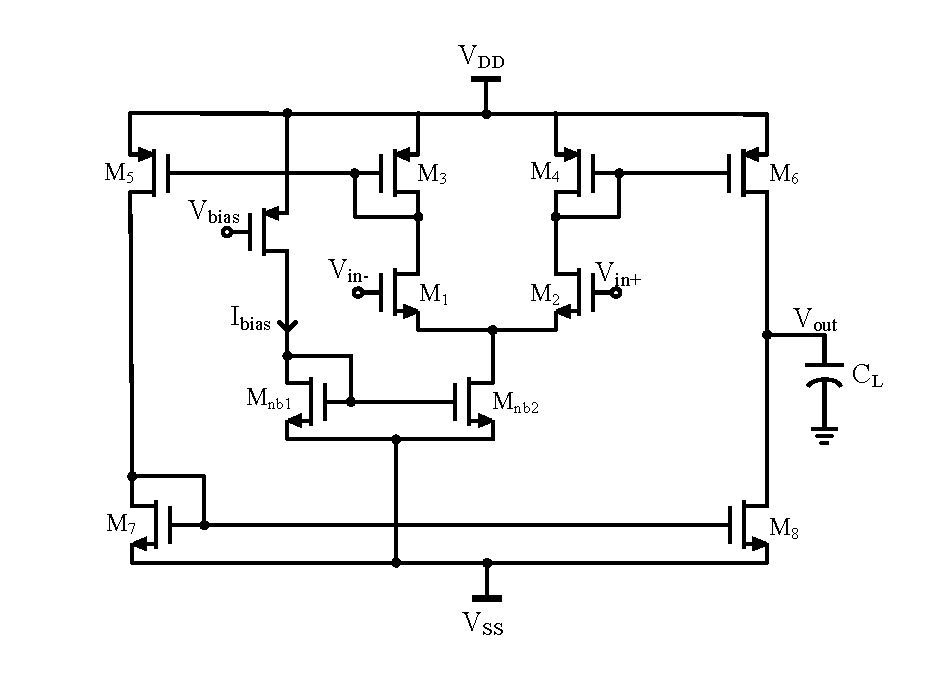
\includegraphics[scale=1]{Figures/Schematics/OTA_NMOS_Vbias.pdf}
\caption{Schematic of the OTA Designed}
\end{figure}

\begin{table} [H]
\centering
\begin{tabular}{@{}cccc@{}}
\toprule
Transistor			& Width				& Length			& Multiplier \\ \midrule
M1					& 8u				& 500n				& 5			\\
M2					& 8u				& 500n				& 5			\\
M3					& 35u				& 500n				& 1			\\
M4					& 35u				& 500n				& 1			\\
M5					& 28u				& 500n				& 3			\\
M6					& 35u				& 500n				& 3			\\
M7					& 35u				& 500n				& 18		\\
M8					& 33u				& 500n				& 18		\\
M9					& 10u				& 500n				& 4			\\
MnB1				& 20u				& 500n				& 8			\\
MnB2				& 20u				& 500n				& 8			\\
\bottomrule
\end{tabular}
\caption{Dimensions of the Transistors of the designed OTA}
\end{table}

\subsection{Test Setup}
\subsubsection{DC Analysis}
\begin{figure} [H]
\centering
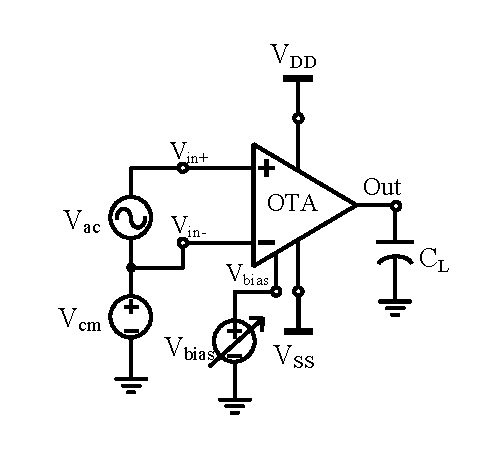
\includegraphics[scale=1]{Figures/Test_Benches/OTA/OTA_ACDC.pdf}
\caption{OTA Test setup for AC, DC and Noise Analysis}
\end{figure}

\begin{table} [H]
\centering
\begin{tabular}{@{}cccccccc@{}}
\toprule
Vbias (mV)					& 150		& 200			& 300			& 400			& 500			& 600			& 700 \\ \midrule
Output DC Bias (mV)			& 13.68		& -16.43		& -78.96		& -144.6		& -213.3		& -285.2		& -360.3 \\
\bottomrule
\end{tabular}
\caption{Output DC Bias Point of the OTA}
\end{table}

\subsubsection{AC Analysis}
\begin{figure} [H]
\centering
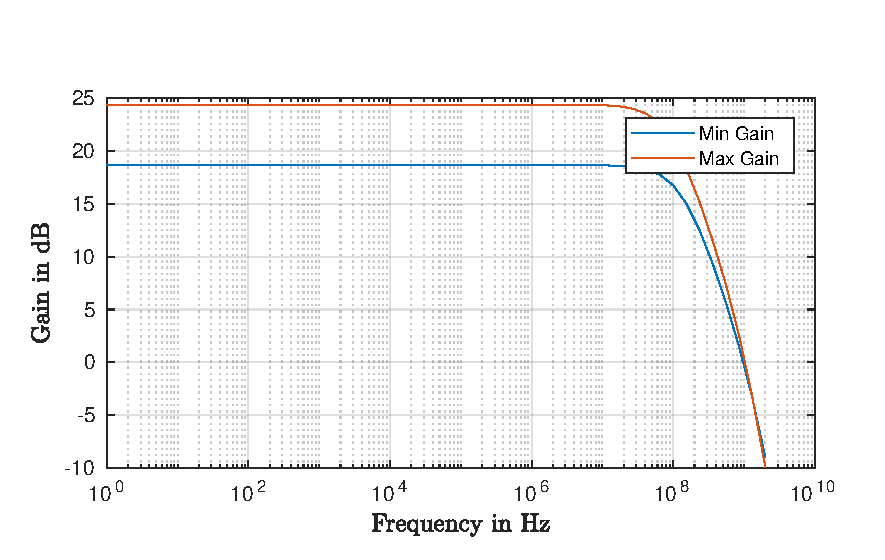
\includegraphics[scale=1]{Figures/Plots/OTA_Gain.pdf}
\caption{OTA Plot of Gain vs Frequency for different Vbias}
\end{figure}

\begin{table} [H]
\centering
\begin{tabular}{@{}cccccccc@{}}
\toprule
Vbias (mV)					& 150		& 200		& 300		& 400		& 500		& 600		& 700 \\ \midrule
Open Loop Gain (dB)			& 18.64		& 19.46		& 20.9		& 22.05		& 22.96		& 23.7		& 24.35 \\
Phase Margin (degrees)		& 63.3		& 60.63		& 55.96		& 52.42		& 49.91		& 48.12		& 46.72 \\
Bandwidth (MHz)				& 135		& 130.7		& 122.2		& 113.7		& 105		& 96.63		& 89.19 \\
\bottomrule
\end{tabular}
\caption{Open Loop Gain, Phase Margin and Bandwidth of the OTA}
\end{table}

\begin{figure} [H]
\centering
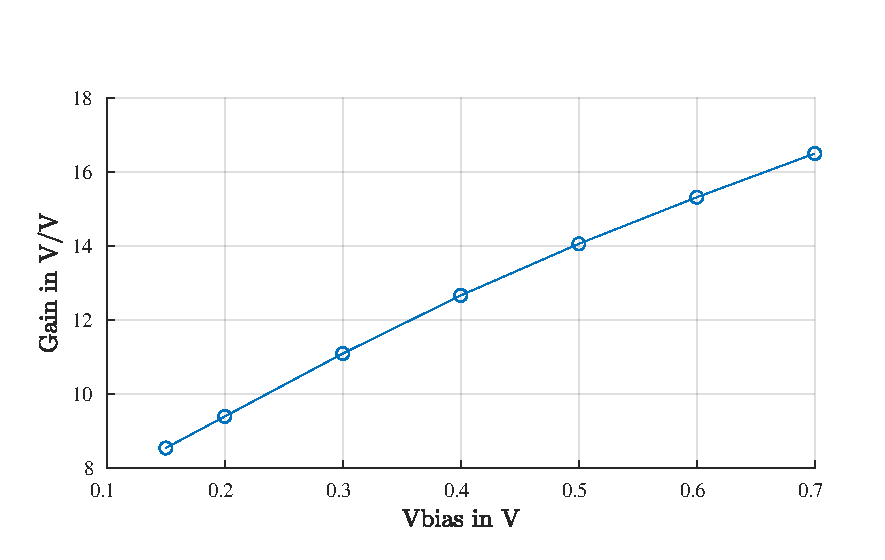
\includegraphics[scale=1]{Figures/Plots/OTA_Gain_Abs.pdf}
\caption{OTA Plot of Gain vs Vbias}
\end{figure}

\begin{table} [H]
\centering
\begin{tabular}{@{}cccccccc@{}}
\toprule
Vbias (mV)					& 150			& 200			& 300			& 400			& 500			& 600			& 700 \\ \midrule
DC Gain (V/V)			& 8.548		& 9.4		& 11.1		& 12.67		& 14.06		& 15.31		& 16.49 \\
\bottomrule
\end{tabular}
\caption{Absolute values of DC Gain of the OTA}
\end{table}

\subsubsection{Noise Analysis}
\begin{table} [H]
\centering
\begin{tabular}{@{}cccccccc@{}}
\toprule
Vbias (mV)					& 150			& 200			& 300			& 400			& 500			& 600			& 700 \\ \midrule
Input Referred Noise (nV/sqrt(Hz))			& 46.36		& 43.73		& 39.83		& 37.29		& 35.57		& 34.31		& 33.28 \\
\bottomrule
\end{tabular}
\caption{Input Referred Noise of the OTA}
\end{table}

\subsubsection{Transient Analysis - Sine Input}
\begin{figure} [H]
\centering
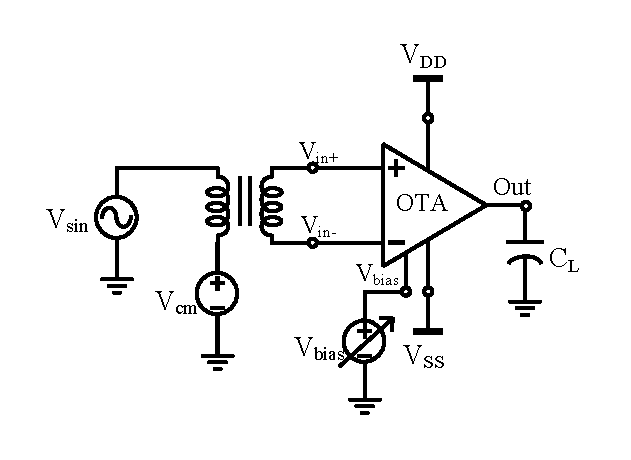
\includegraphics[scale=1]{Figures/Test_Benches/OTA/OTA_Sine.pdf}
\caption{OTA Test setup for Transient Analysis - Sine Wave Input}
\end{figure}

\begin{figure} [H]
\centering
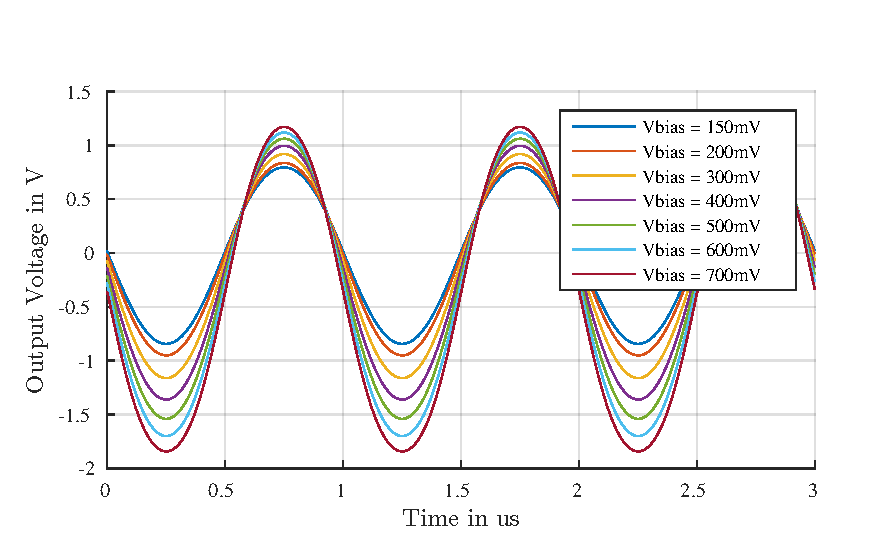
\includegraphics[scale=1]{Figures/Plots/OTA_Sine.pdf}
\caption{OTA Output Voltage for vs time for different Vbias}
\end{figure}

\begin{table} [H]
\centering
\begin{tabular}{@{}cccccccc@{}}
\toprule
Vbias (mV)					& 150			& 200			& 300			& 400			& 500			& 600			& 700 \\ \midrule
Vout Max (V)			& 0.7949		& 0.8362		& 0.9188		& 0.995		& 1.061		& 1.119		& 1.172 \\
Vout Min (V)			& -0.844		& -0.9505		& -1.162		& -1.361		& -1.54		& -1.7		& -1.842 \\
Vout Swing (V)				& 1.639		& 1.787		& 2.081		& 2.356		& 2.601		& 2.818		& 3.014 \\
HD2 (dBc) 				& -44.83		& -44.28		& -43.86		& -44.74		& -47.97		& -60.86		& -48.75 \\
HD3 (dBc) 				& -52.15		& -49.69		& -46.13		& -43.87		& -42.24		& -40.78		& -39.32 \\
\bottomrule
\end{tabular}
\caption{Transient Parameters of the OTA}
\end{table}

\subsubsection{Transient Analysis - Square Input}
\begin{figure} [H]
\centering
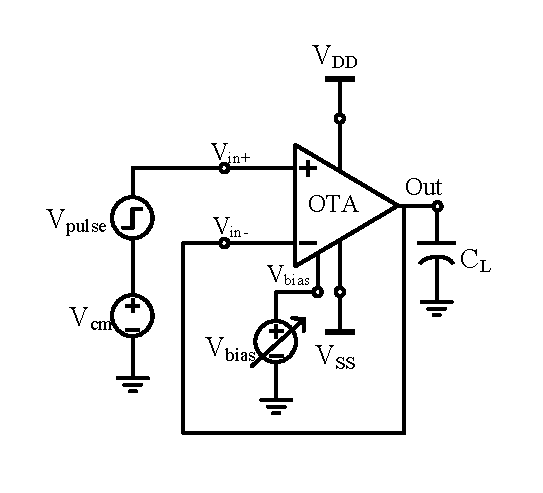
\includegraphics[scale=1]{Figures/Test_Benches/OTA/OTA_Slew.pdf}
\caption{OTA Test setup for Transient Analysis - Square Wave Input}
\end{figure}

\begin{table} [H]
\centering
\begin{tabular}{@{}cccccccc@{}}
\toprule
Vbias (mV)					& 150			& 200			& 300			& 400			& 500			& 600			& 700 \\ \midrule
Slew Rate Rising Edge (V/us)			& 386.9		& 407.8		& 452.9		& 501.9 	& 547.6		& 585.4		& 609.3 \\
Slew Rate Falling Edge (V/us)			& -389		& -413.8		& -469.4		& -523.5		& -570.5		& -605.7		& -626.4 \\
\bottomrule
\end{tabular}
\caption{Slew Rate of the OTA}
\end{table}

\subsubsection{AC Analysis - PSRR}
\begin{figure} [H]
\centering
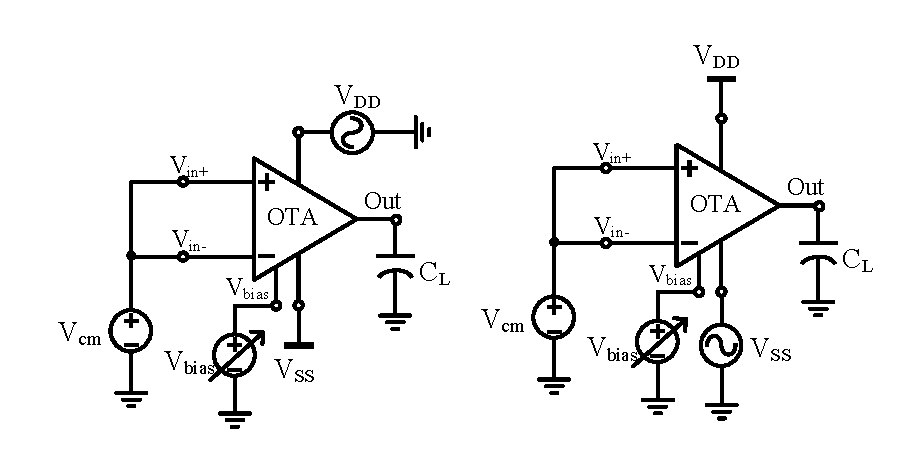
\includegraphics[scale=1]{Figures/Test_Benches/OTA/OTA_PSRR.pdf}
\caption{OTA Test setup for calculating PSRR}
\end{figure}

\begin{table} [H]
\centering
\begin{tabular}{@{}cccccccc@{}}
\toprule
Vbias (mV)					& 150			& 200			& 300			& 400			& 500			& 600			& 700 \\ \midrule
PSRR (VDD Supply) (nA/V)			& 234.6		& 236.9		& 241.6		& 246.7 	& 252.2		& 258		& 264.3 \\
PSRR (VSS Supply) (nA/V)			& 254.5		& 256.5		& 260.4		& 264.2		& 267.9		& 271.5		& 274.9 \\
\bottomrule
\end{tabular}
\caption{Power Supply Rejection Ratio of the OTA}
\end{table}

\subsubsection{AC Analysis - Input Impedance}
\begin{figure} [H]
\centering
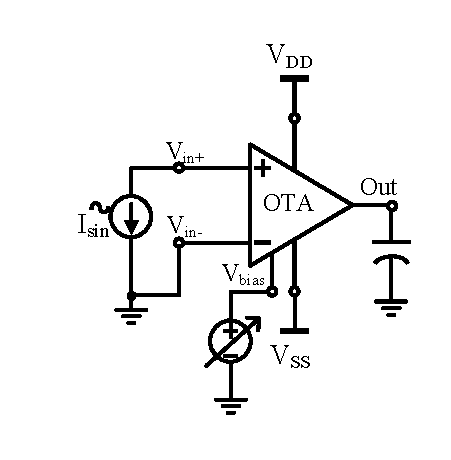
\includegraphics[scale=1]{Figures/Test_Benches/OTA/OTA_Zin.pdf}
\caption{OTA Test setup for calculating Input Impedance}
\end{figure}

\begin{table} [H]
\centering
\begin{tabular}{@{}cccccccc@{}}
\toprule
Vbias (mV)					& 150		& 200			& 300			& 400			& 500			& 600			& 700 \\ \midrule
Input Impedance (Mega Ohms)			& 3.38		& 3.388		& 3.403		& 3.419		& 3.434		& 3.45		& 3.467 \\
\bottomrule
\end{tabular}
\caption{Input Impedance of the OTA}
\end{table}

\subsubsection{AC Analysis - Output Impedance}
\begin{figure} [H]
\centering
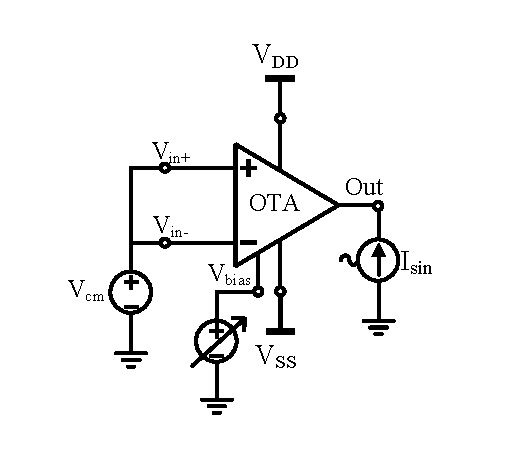
\includegraphics[scale=1]{Figures/Test_Benches/OTA/OTA_Zout.pdf}
\caption{OTA Test setup for calculating Output Impedance}
\end{figure}

\begin{table} [H]
\centering
\begin{tabular}{@{}cccccccc@{}}
\toprule
Vbias (mV)					& 150		& 200			& 300			& 400			& 500			& 600			& 700 \\ \midrule
Input Impedance (kilo Ohms)			& 1.262		& 1.3		& 1.382		& 1.473		& 1.577		& 1.697		& 1.837 \\
\bottomrule
\end{tabular}
\caption{Output Impedance of the OTA}
\end{table}

\section{OP AMP Design}

\subsection{Schematic}
\begin{figure} [H]
\centering
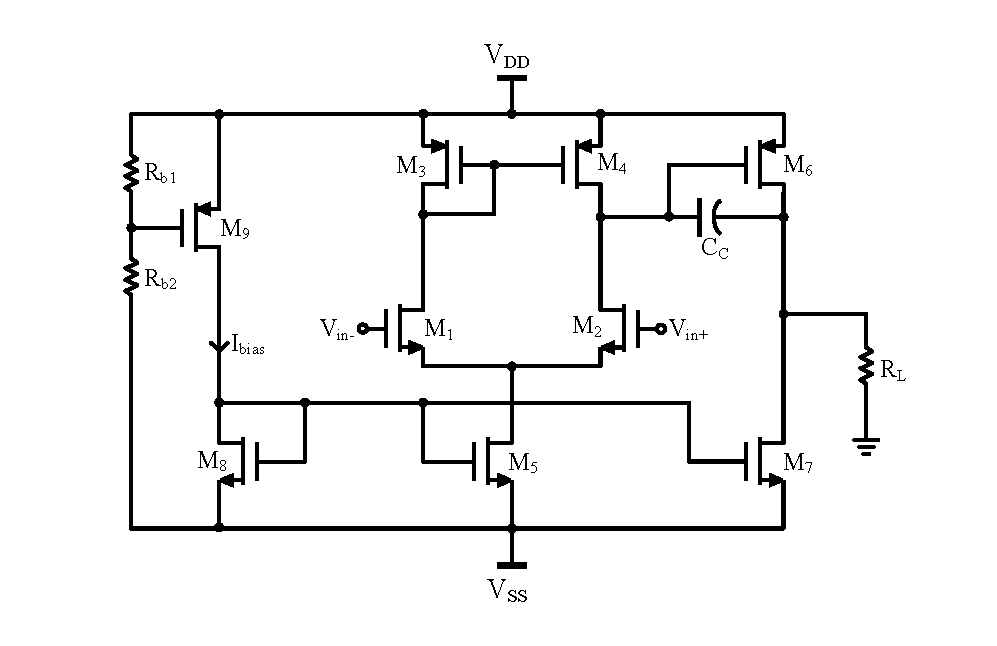
\includegraphics[scale=1]{Figures/Schematics/OPAMP_Vbias.pdf}
\caption{Schematic of the OPAMP Designed}
\end{figure}

\begin{table} [H]
\centering
\begin{tabular}{@{}cccc@{}}
\toprule
Transistor			& Width				& Length			& Multiplier \\ \midrule
M1					& 5u				& 500n				& 2			\\
M2					& 5u				& 500n				& 2			\\ 
M3					& 30u				& 500n				& 1			\\
M4					& 30u				& 500n				& 1			\\ 
M5					& 2u				& 500n				& 1			\\
M6					& 85u				& 500n				& 55		\\ 
M7					& 50u				& 500n				& 48		\\
M8					& 2u				& 500n				& 1			\\ 
M9					& 700n				& 500n				& 1			\\
 
\bottomrule
\end{tabular}
\caption{Dimensions of the Transistors of the designed OPAMP}
\end{table}

\subsection{Test Setup}

\begin{figure} [H]
\centering
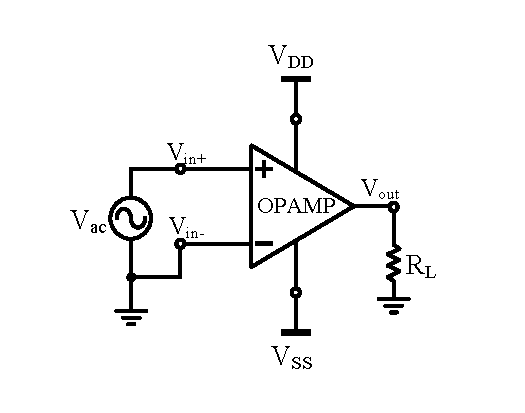
\includegraphics[scale=1]{Figures/Test_Benches/OPAMP/OPAMP_ACDC.pdf}
\caption{OPAMP Test setup for AC, DC and Noise Analysis}
\end{figure}

\begin{figure} [H]
\centering
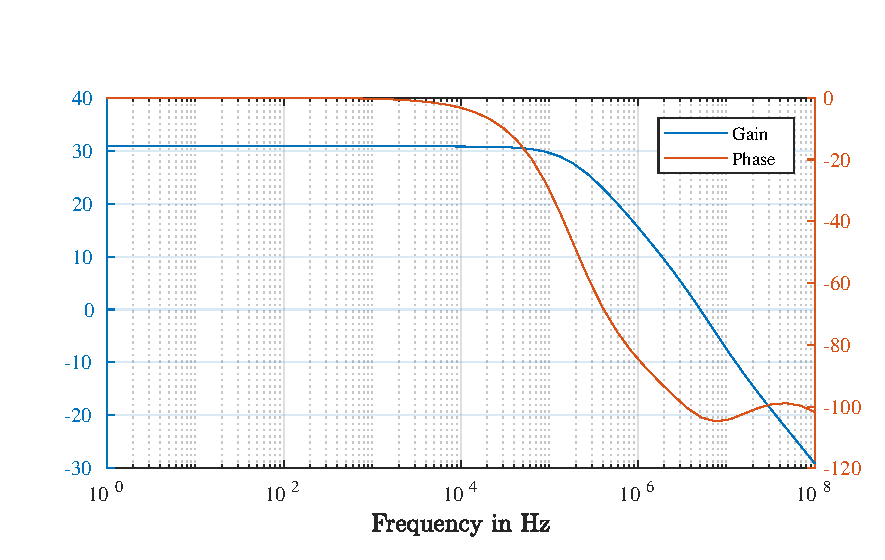
\includegraphics[scale=1]{Figures/Plots/OPAMP_Gain_PM.pdf}
\caption{OPAMP Plot of Gain and Phase vs Frequency}
\end{figure}

\begin{figure} [H]
\centering
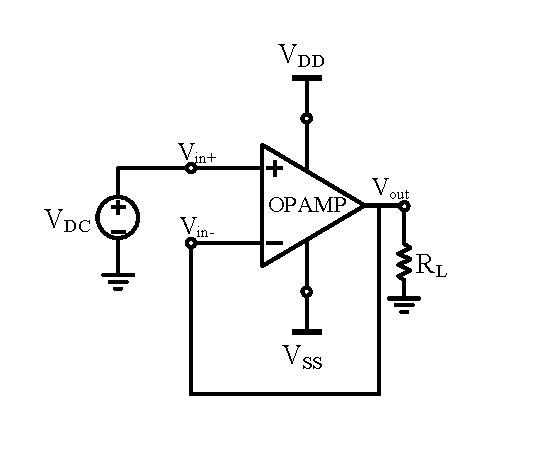
\includegraphics[scale=1]{Figures/Test_Benches/OPAMP/OPAMP_ICMR.pdf}
\caption{OPAMP Test setup for calculating ICMR}
\end{figure}

\begin{figure} [H]
\centering
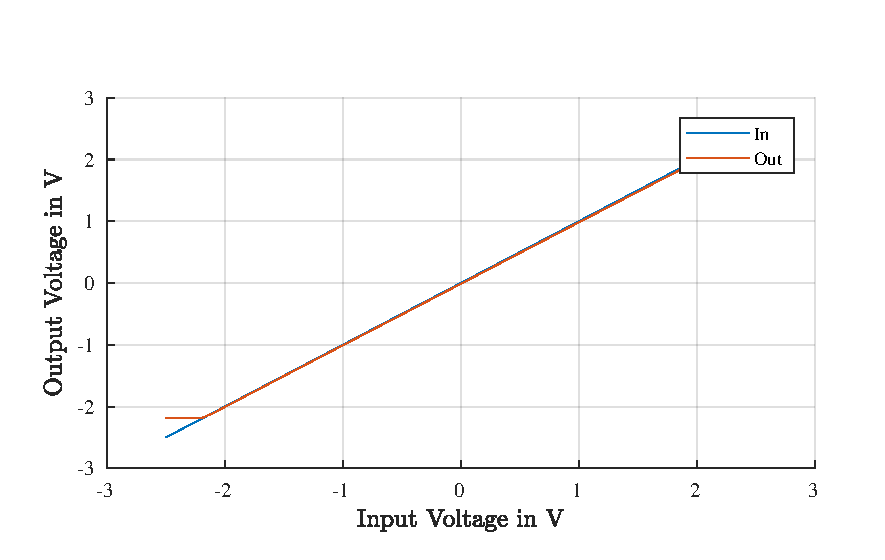
\includegraphics[scale=1]{Figures/Plots/OPAMP_ICMR.pdf}
\caption{OPAMP Plot of ICMR vs Vin}
\end{figure}

\begin{figure} [H]
\centering
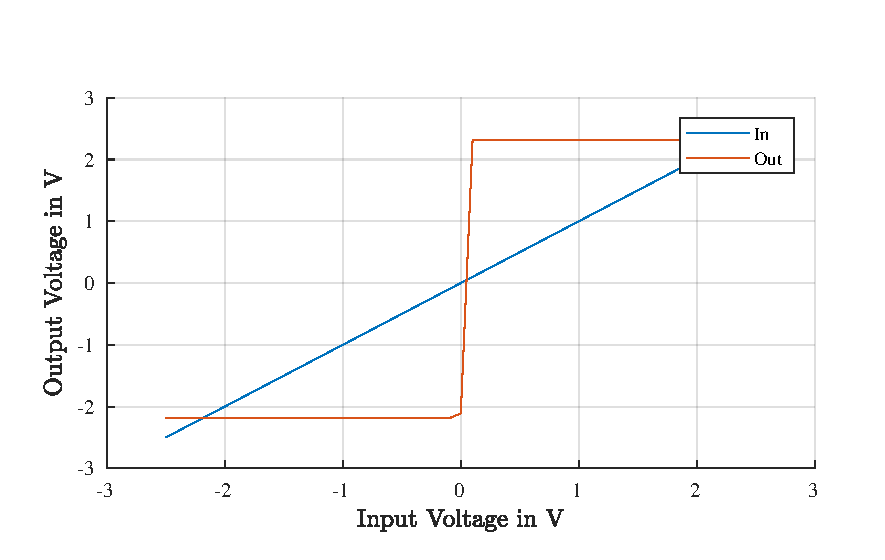
\includegraphics[scale=1]{Figures/Plots/OPAMP_OutSwing.pdf}
\caption{OPAMP Plot of Output Voltage Swing vs Vin}
\end{figure}

\begin{figure} [H]
\centering
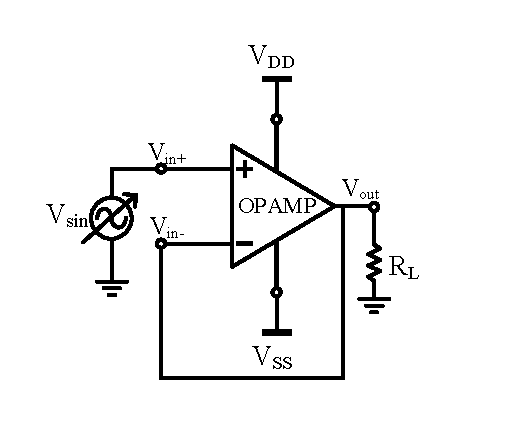
\includegraphics[scale=1]{Figures/Test_Benches/OPAMP/OPAMP_Sine.pdf}
\caption{Test setup for Transient Analysis - Sine Wave Input}
\end{figure}

\begin{figure} [H]
\centering
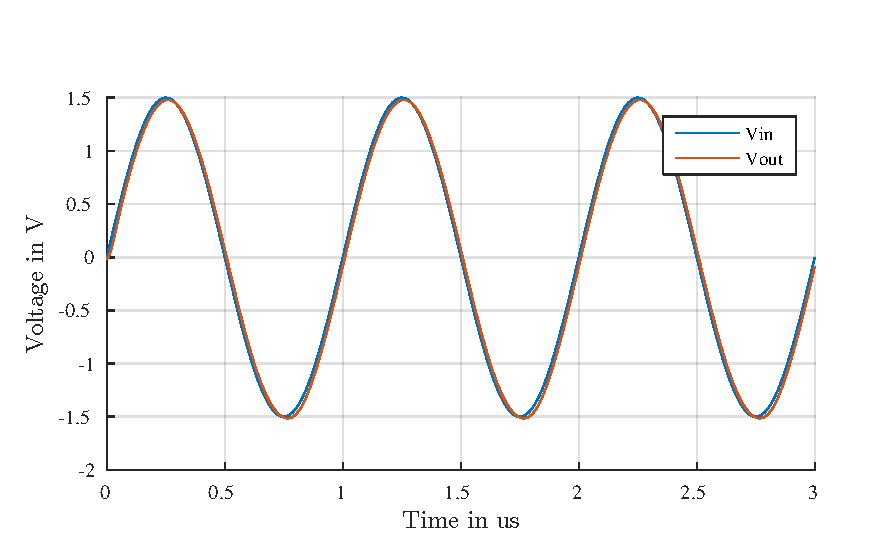
\includegraphics[scale=1]{Figures/Plots/OPAMP_Buffer.pdf}
\caption{OPAMP Plot of Output Voltage vs time}
\end{figure}

\begin{figure} [H]
\centering
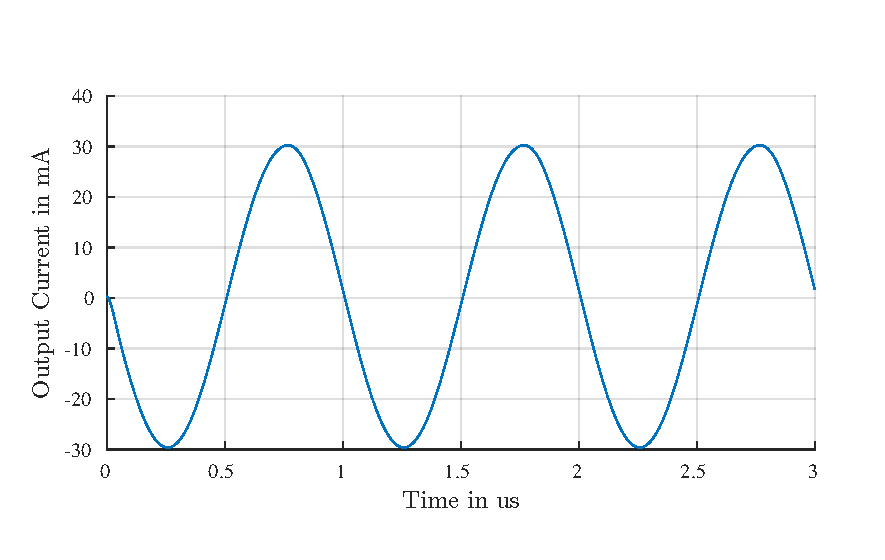
\includegraphics[scale=1]{Figures/Plots/OPAMP_Iout.pdf}
\caption{OPAMP Plot of Ourput Current vs time}
\end{figure}

\begin{figure} [H]
\centering
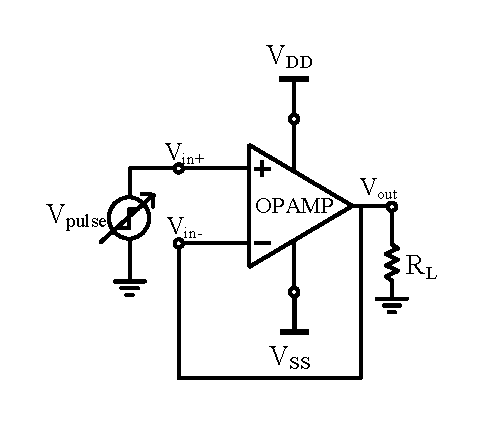
\includegraphics[scale=1]{Figures/Test_Benches/OPAMP/OPAMP_Slew.pdf}
\caption{Test setup for Transient Analysis - Square Wave Input}
\end{figure}

\begin{figure} [H]
\centering
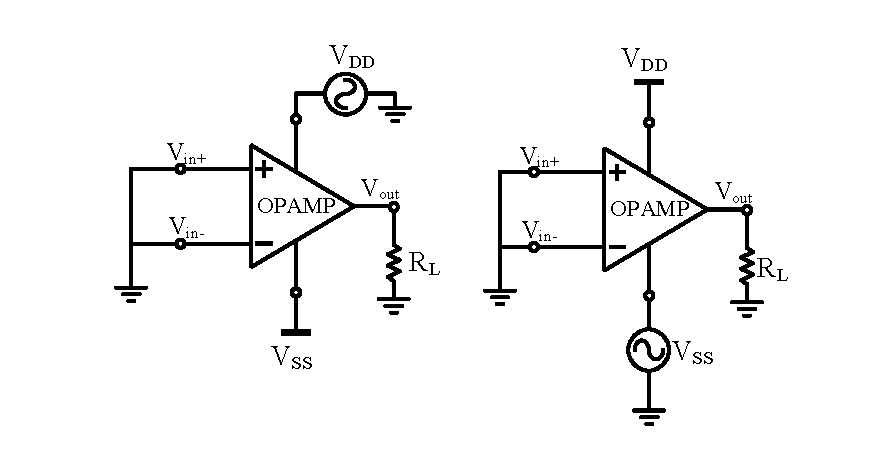
\includegraphics[scale=1]{Figures/Test_Benches/OPAMP/OPAMP_PSRR.pdf}
\caption{Test setup for calculating PSRR}
\end{figure}

\begin{figure} [H]
\centering
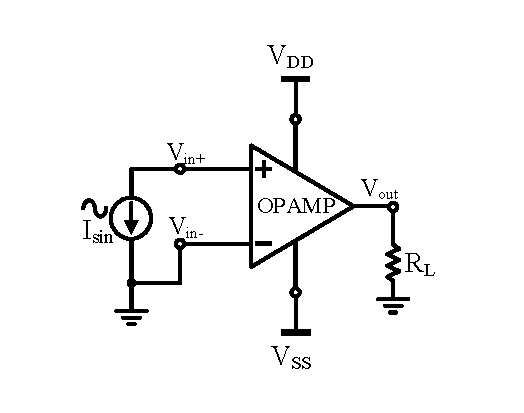
\includegraphics[scale=1]{Figures/Test_Benches/OPAMP/OPAMP_Zin.pdf}
\caption{Test setup for calculating Input Impedance}
\end{figure}

\begin{figure} [H]
\centering
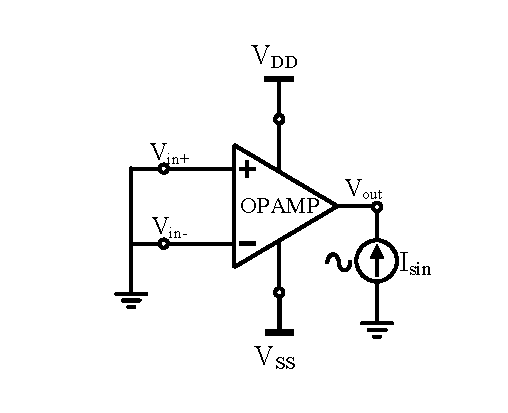
\includegraphics[scale=1]{Figures/Test_Benches/OPAMP/OPAMP_Zout.pdf}
\caption{Test setup for calculating Output Impedance}
\end{figure}

\begin{table} [H]
\centering
\begin{tabular}{@{}cc@{}}
\toprule
Parameter					& Value				\\ \midrule
Open Loop Gain				& 30.8 dB			\\
Gain Bandwidth Product		& 6.2 MHz			\\
Phase Margin				& 76.79				\\
ICMR (min)					& -2.19 V			\\
ICMR (max)					& 2.089 V			\\
Output Current (max)		& -29.6 mA			\\
Output Current (min)		& 30.28 mA			\\
Output Voltage Swing		& -2.19 .. 2.089 	\\
Slew Rate					& 10 V/us			\\
PSRR (VDD)					& 30.96 uA/V		\\
PSRR (VSS)					& 138.8 uA/V		\\
Input Impedance				& 9.04 MOhms		\\
Output Impedance			& 4.167 Ohms		\\
\bottomrule
\end{tabular}
\caption{Simlation Results of the OPAMP}
\end{table}

\section{The Complete Design}

\begin{figure} [H]
\centering
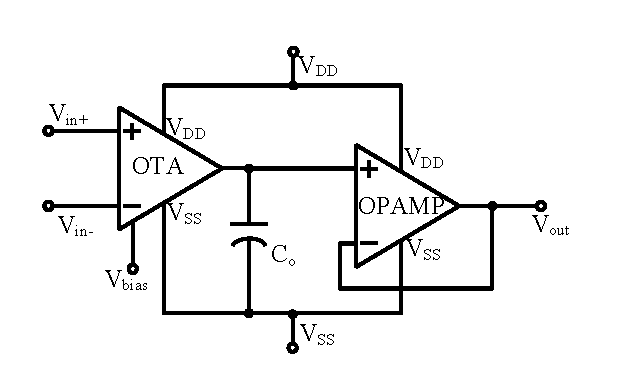
\includegraphics[scale=1]{Figures/System_Level/System_Overview.pdf}
\caption{Block Diagram of the Overall System}
\end{figure}

\begin{figure} [H]
\centering
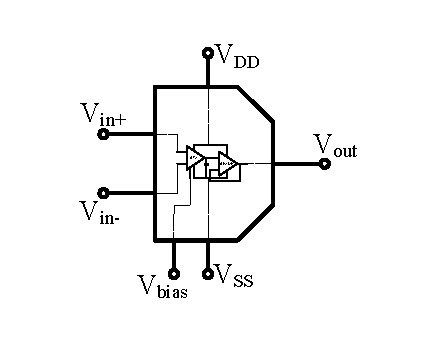
\includegraphics[scale=1]{Figures/System_Level/System_Symbol.pdf}
\caption{Schematic Symbol for the Overall System}
\end{figure}

\subsection{Schematic}

\begin{figure} [H]
\centering
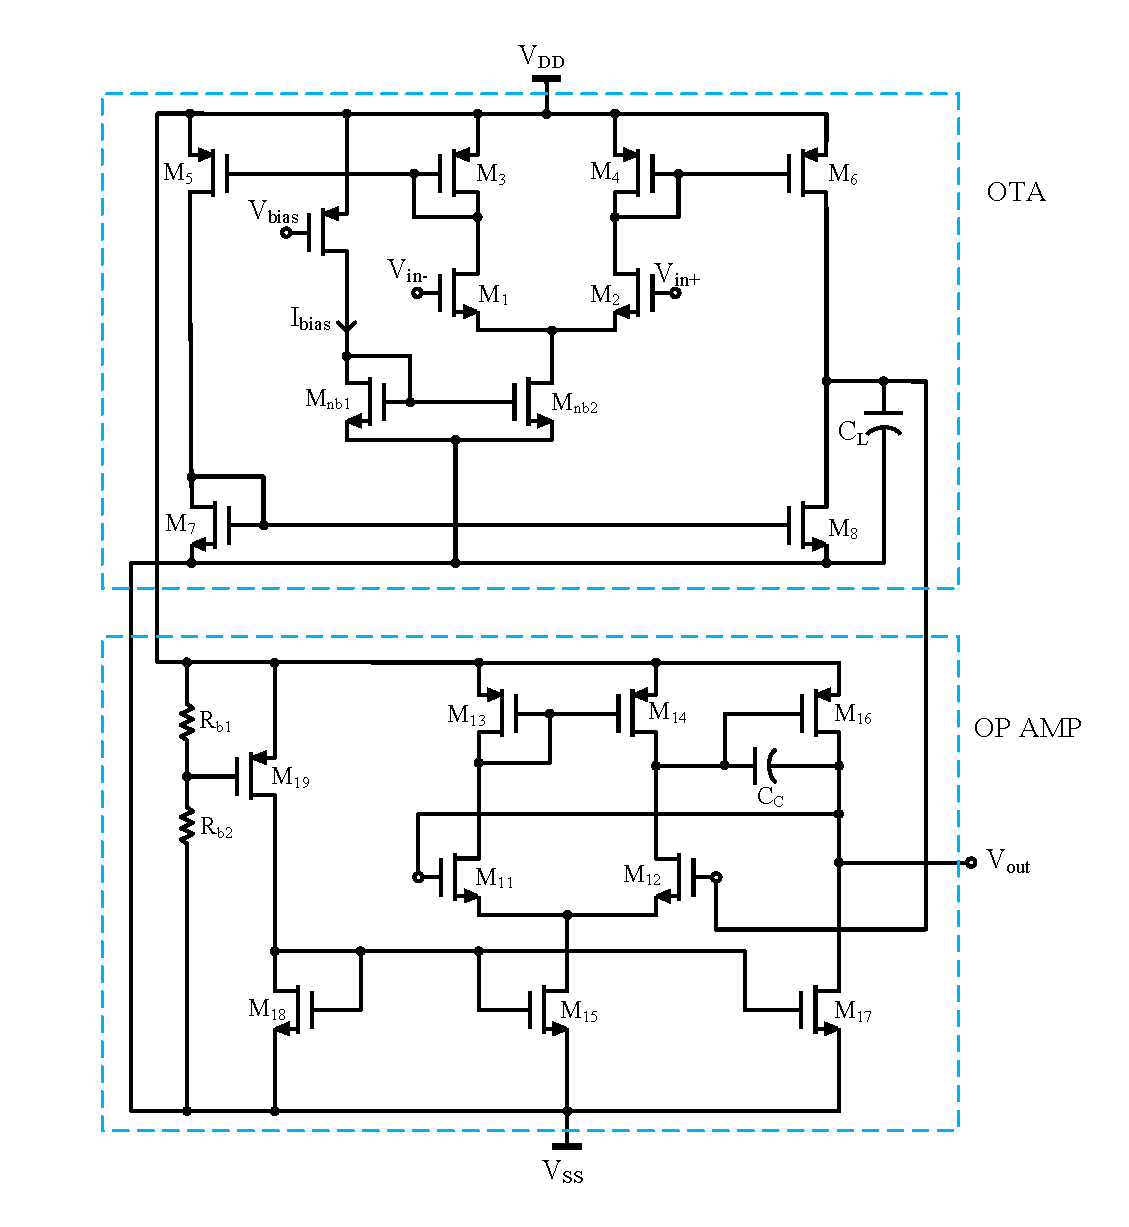
\includegraphics[scale=1]{Figures/Schematics/OTA_OPAMP_Schematic.pdf}
\caption{Schematic Diagram for the Overall System}
\end{figure}
